\documentclass[12pt,letterpaper]{article}
\usepackage{fullpage}
\usepackage[top=2cm, bottom=4.5cm, left=2.5cm, right=2.5cm]{geometry}
\usepackage{amsmath,amsthm,amsfonts,amssymb,amscd}
\usepackage{lastpage}
\usepackage{enumerate}
\usepackage{fancyhdr}
\usepackage{hyperref}
\usepackage{pythontex}
\usepackage[siunitx]{circuitikz}
\usepackage{xcolor}
\usepackage[inline]{enumitem}
\usepackage{booktabs}
\usepackage{relsize}
\usepackage{calculator}
\usepackage{siunitx}

\setlength{\parindent}{0.0in}
\setlength{\parskip}{0.05in}

% Edit these as appropriate
\newcommand\course{MCEN 5228-004}
\newcommand\project{2}                  % <-- homework number
\newcommand\NetIDa{Coovi Meha}           % <-- NetID of person #1
\newcommand\NetIDb{MEid:481-473}           % <-- NetID of person #2 (Comment this line out for problem sets)

\pagestyle{fancyplain}
\headheight 35pt
\lhead{\NetIDa}
\lhead{\NetIDa\\\NetIDb}                 % <-- Comment this line out for problem sets (make sure you are person #1)
\chead{\textbf{\Large Project \project}}
\rhead{\course \\ \today}
\lfoot{}
\cfoot{}
\rfoot{\small\thepage}
\headsep 1.5em
\begin{document}
\begin{pycode}
R=5100
C=2.2*10**-6
tau=2/(R*C)
tau1=0.5*tau
omega=tau**0.5
\end{pycode}
\section*{Abstract}
In system analysis, engineers study the performance of a system using theoretical and 
experimental approaches. However, most system do not perform as  predicted by the theoretical model. Thus, 
the need to improve the system performance. In this project, we analyse the performance of 
and closed loop circuit using MyRio and an RRC circuit by sending a step input of 1 to the 
system.   
\section*{Backgrounds}
This experiment used an RRC circuit as showed bellow. 
\begin{figure}[h]
    \begin{center}
        \begin{circuitikz}\draw
            (0,0) to[battery, color=red] (0,4) 
            to[R=5.1<k\ohm>] (4,4) to [R=5.1<k\ohm>] (4,0)
            --(0,0) 
            (4,4) -- (6,4) to[capacitor, C=2.2<\micro\farad>, color=blue] (6,0) 
            -- (4,0) 
            (6,4)  to[short,-*] (8,4) 
            (8,0) to[open, v=${V_out}$, color=red] (8,4) 
            (6,0)  to[short,-*] (8,0) ;
        \end{circuitikz}
        \caption{RRC Circuit}
        \end{center}
\end{figure}
we were interested in measuring the voltage crossing the capacitor and the resistor in parallel.
The measure voltage is compared to the input voltage in oder to analyse the gain of the system, the rise time of, the settle time and others parameters associated
the input-output signal. 
The system was fed with two difference signals:
\begin{itemize}
    \item A step input signal of 1 volt
    \item A sinusoidal input of amplitude 1 volt, phase of zero degree and 10 Hzt frequency 
\end{itemize}
\section*{Experiment Set-up}
Using MyRio, we connected the analog input the pin AI0 and the output
to pin AO1. The feedback was completed by subtracting the input signal
from output and feeding it the system as show by the figure bellow.\\
\begin{figure}[h]
    \centering
    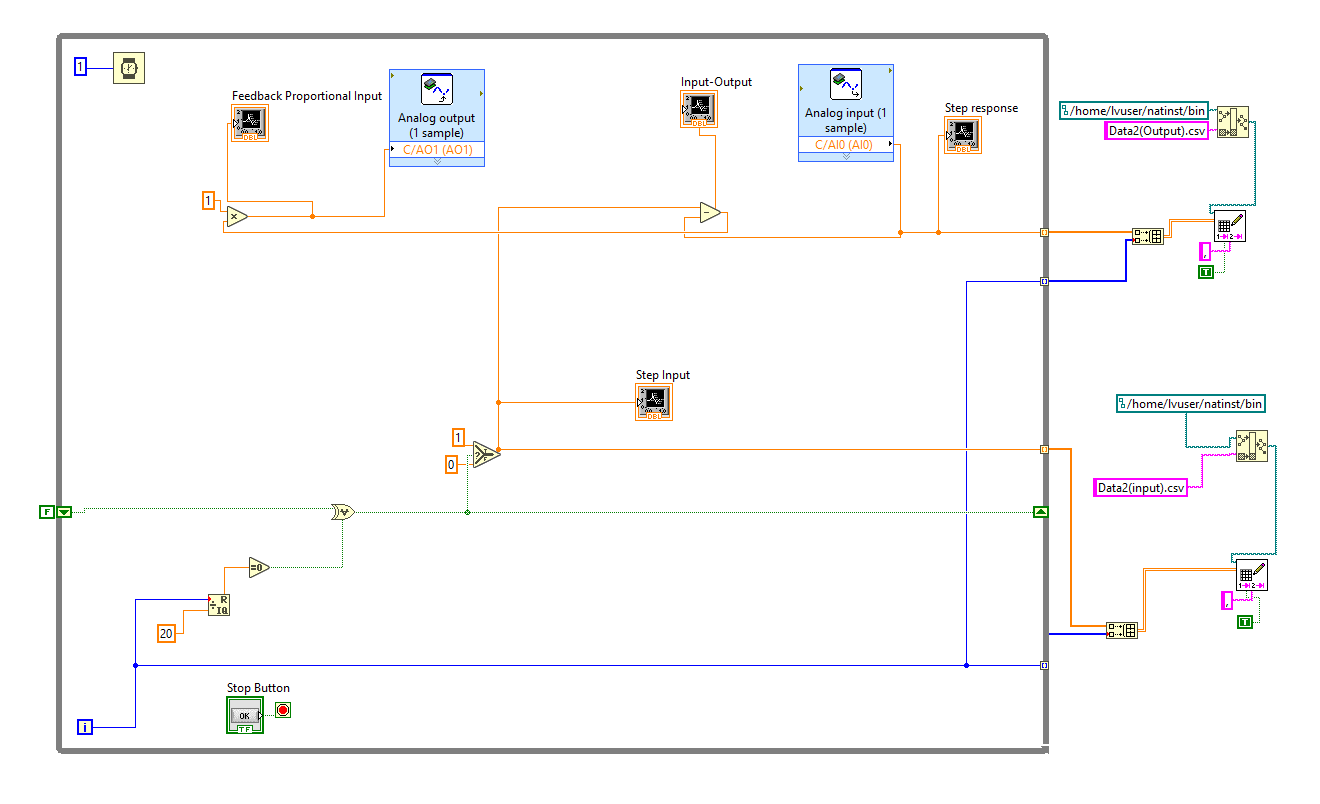
\includegraphics[width=10cm]{Capture.png}
    \caption{Experimental plot of step input of 1 volt to an RRC circuit.}
\end{figure}

The MyRIo integrated to the circuit is showed bellow. MyRio analog input need 
a reference voltage to be able to read the correct input data. Thus, we connected
the +1 pin to the high voltage coming in the device and the -1 to ground.
\begin{figure}[h]
    \centering
    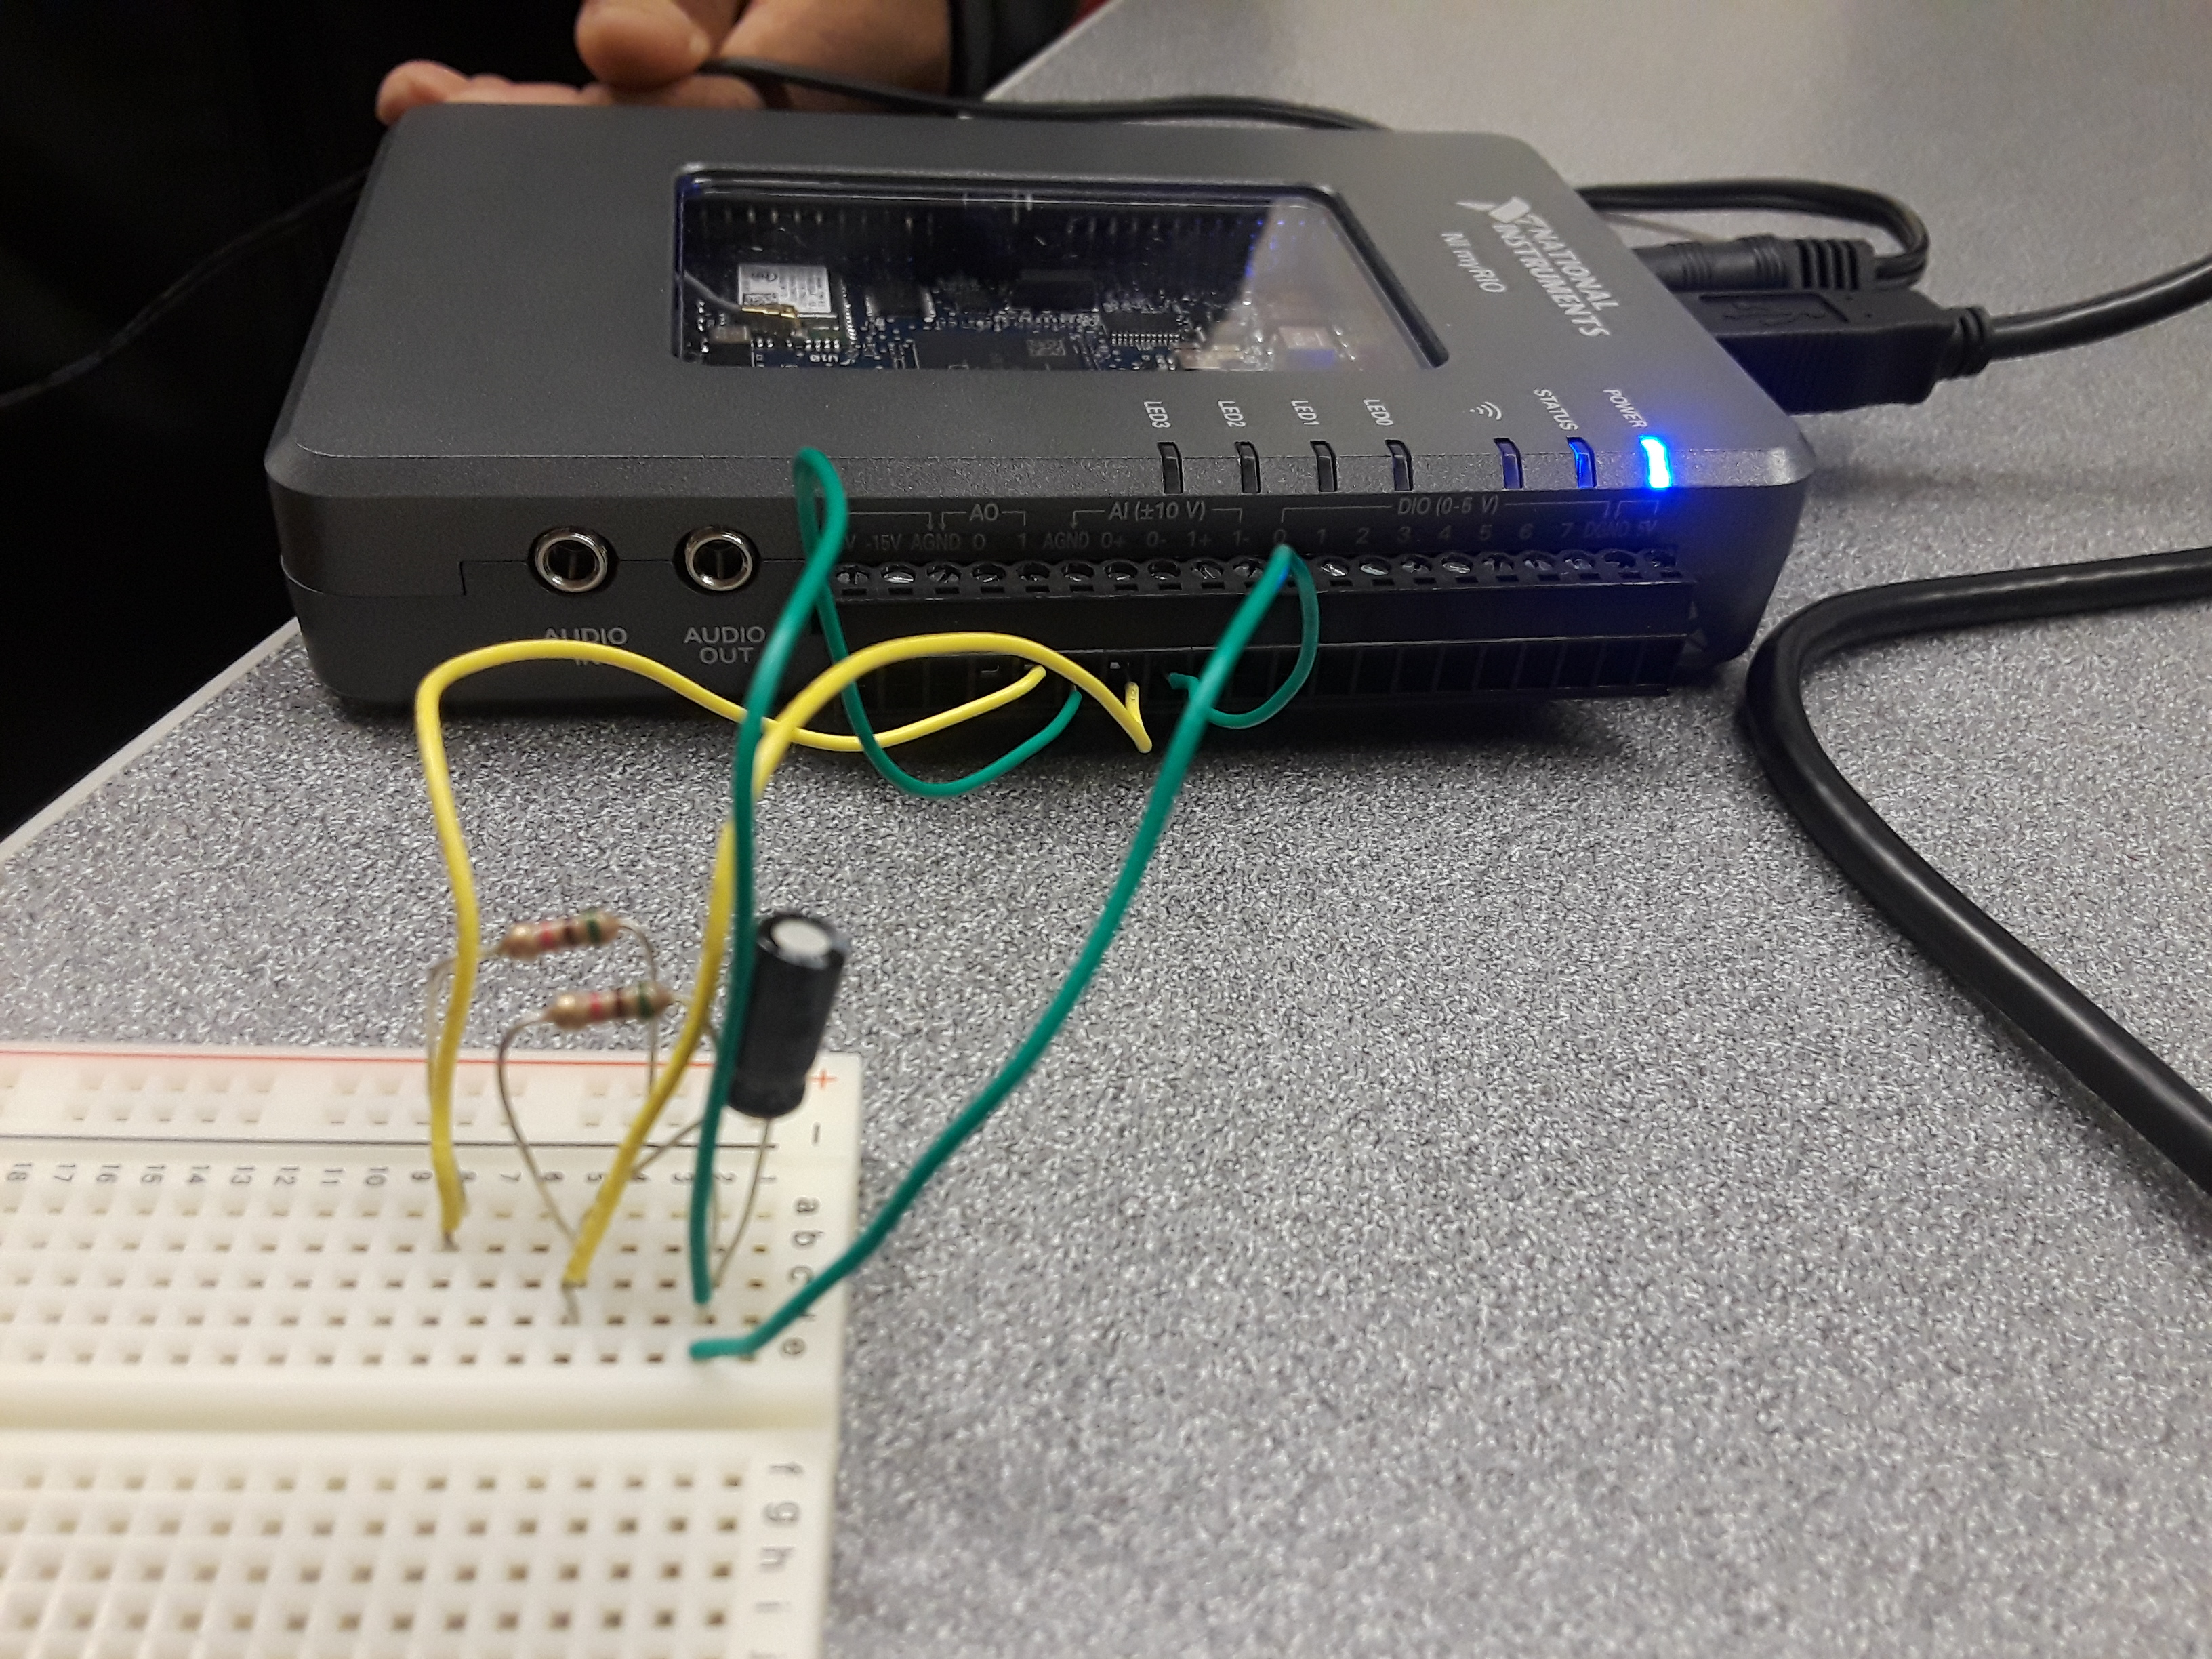
\includegraphics[width=10cm]{20190224_134224.jpg}
    \caption{Experimental plot of step input of 1 volt to an RRC circuit.}
\end{figure}   
\section*{Theoretical Results}
\begin{itemize}
    \item Idealize Elements
    \begin{circuitikz}\draw
        (0,0) node[{label=above:$V_{in}$}]{} to [R=$R$, *-*] node[{label=above:$V_{1}$}]{}(4,0)
        (5,0) node[{label=above:$V_{2}$}]{}to [capacitor=$C$, *-*] node[{label=above:$V_{3}$}]{}(9,0)
         (10,0) node[{label=above:$V_{4}$}]{} to [R=R, *-*] node[{label=above:$V_{5}$}]{}(14,0);
    \end{circuitikz}
    \item  Derivation of opened loop Transfer Function and Time Domain Equation
    From the Idealized element, the idealized formula can be derived as follow.
        \begin{enumerate*}
            \item \(V_{in}-V_{1}= R*I\) \quad \quad \quad \quad
            \item \(V_{2}-V_{3}=\frac{1}{C}*I_{2}\) \quad \quad \quad \quad
            \item \(V_{4}-V_{5}= R*I\) \quad \quad \quad \quad
            \item \(V_{1}=V_{2}=V_{4}=V_{out}\) \quad \quad \quad \quad
            \item \(V_{3}=V_{5}=0\)
        \end{enumerate*}
    From the above equations: 
    \begingroup
    \begin{equation}
        H(s)=\frac{1}{2}  *\frac{\frac{2}{RC}}{s+ \frac{2}{RC}} \quad \equiv \quad H(s)=\frac{\py{round(tau1,2)}}{s+ \py{round(tau,2)}}
    \end{equation}
    \endgroup
    with R=5.1k \({\Omega}\) and C=2.2 \(\si{\micro\farad}\)
    The laplace inverse of the equation (1) leads to:
    \begingroup
        \begin{equation}
            y(t)=\frac{1}{2}({1} - e^{\frac{-2t}{CR}})
        \end{equation}
    \endgroup
    \item Closed loop equation
    \begin{equation}
        G(s)=\frac{KH(s)}{1+kH(s)}
    \end{equation}  
    with k the proportional controller set to 1 during this experiment
    \item step input plot\\
    Using Matlab step function, the plot of the step input is showed below.

    \begin{figure}[h]
        \centering
        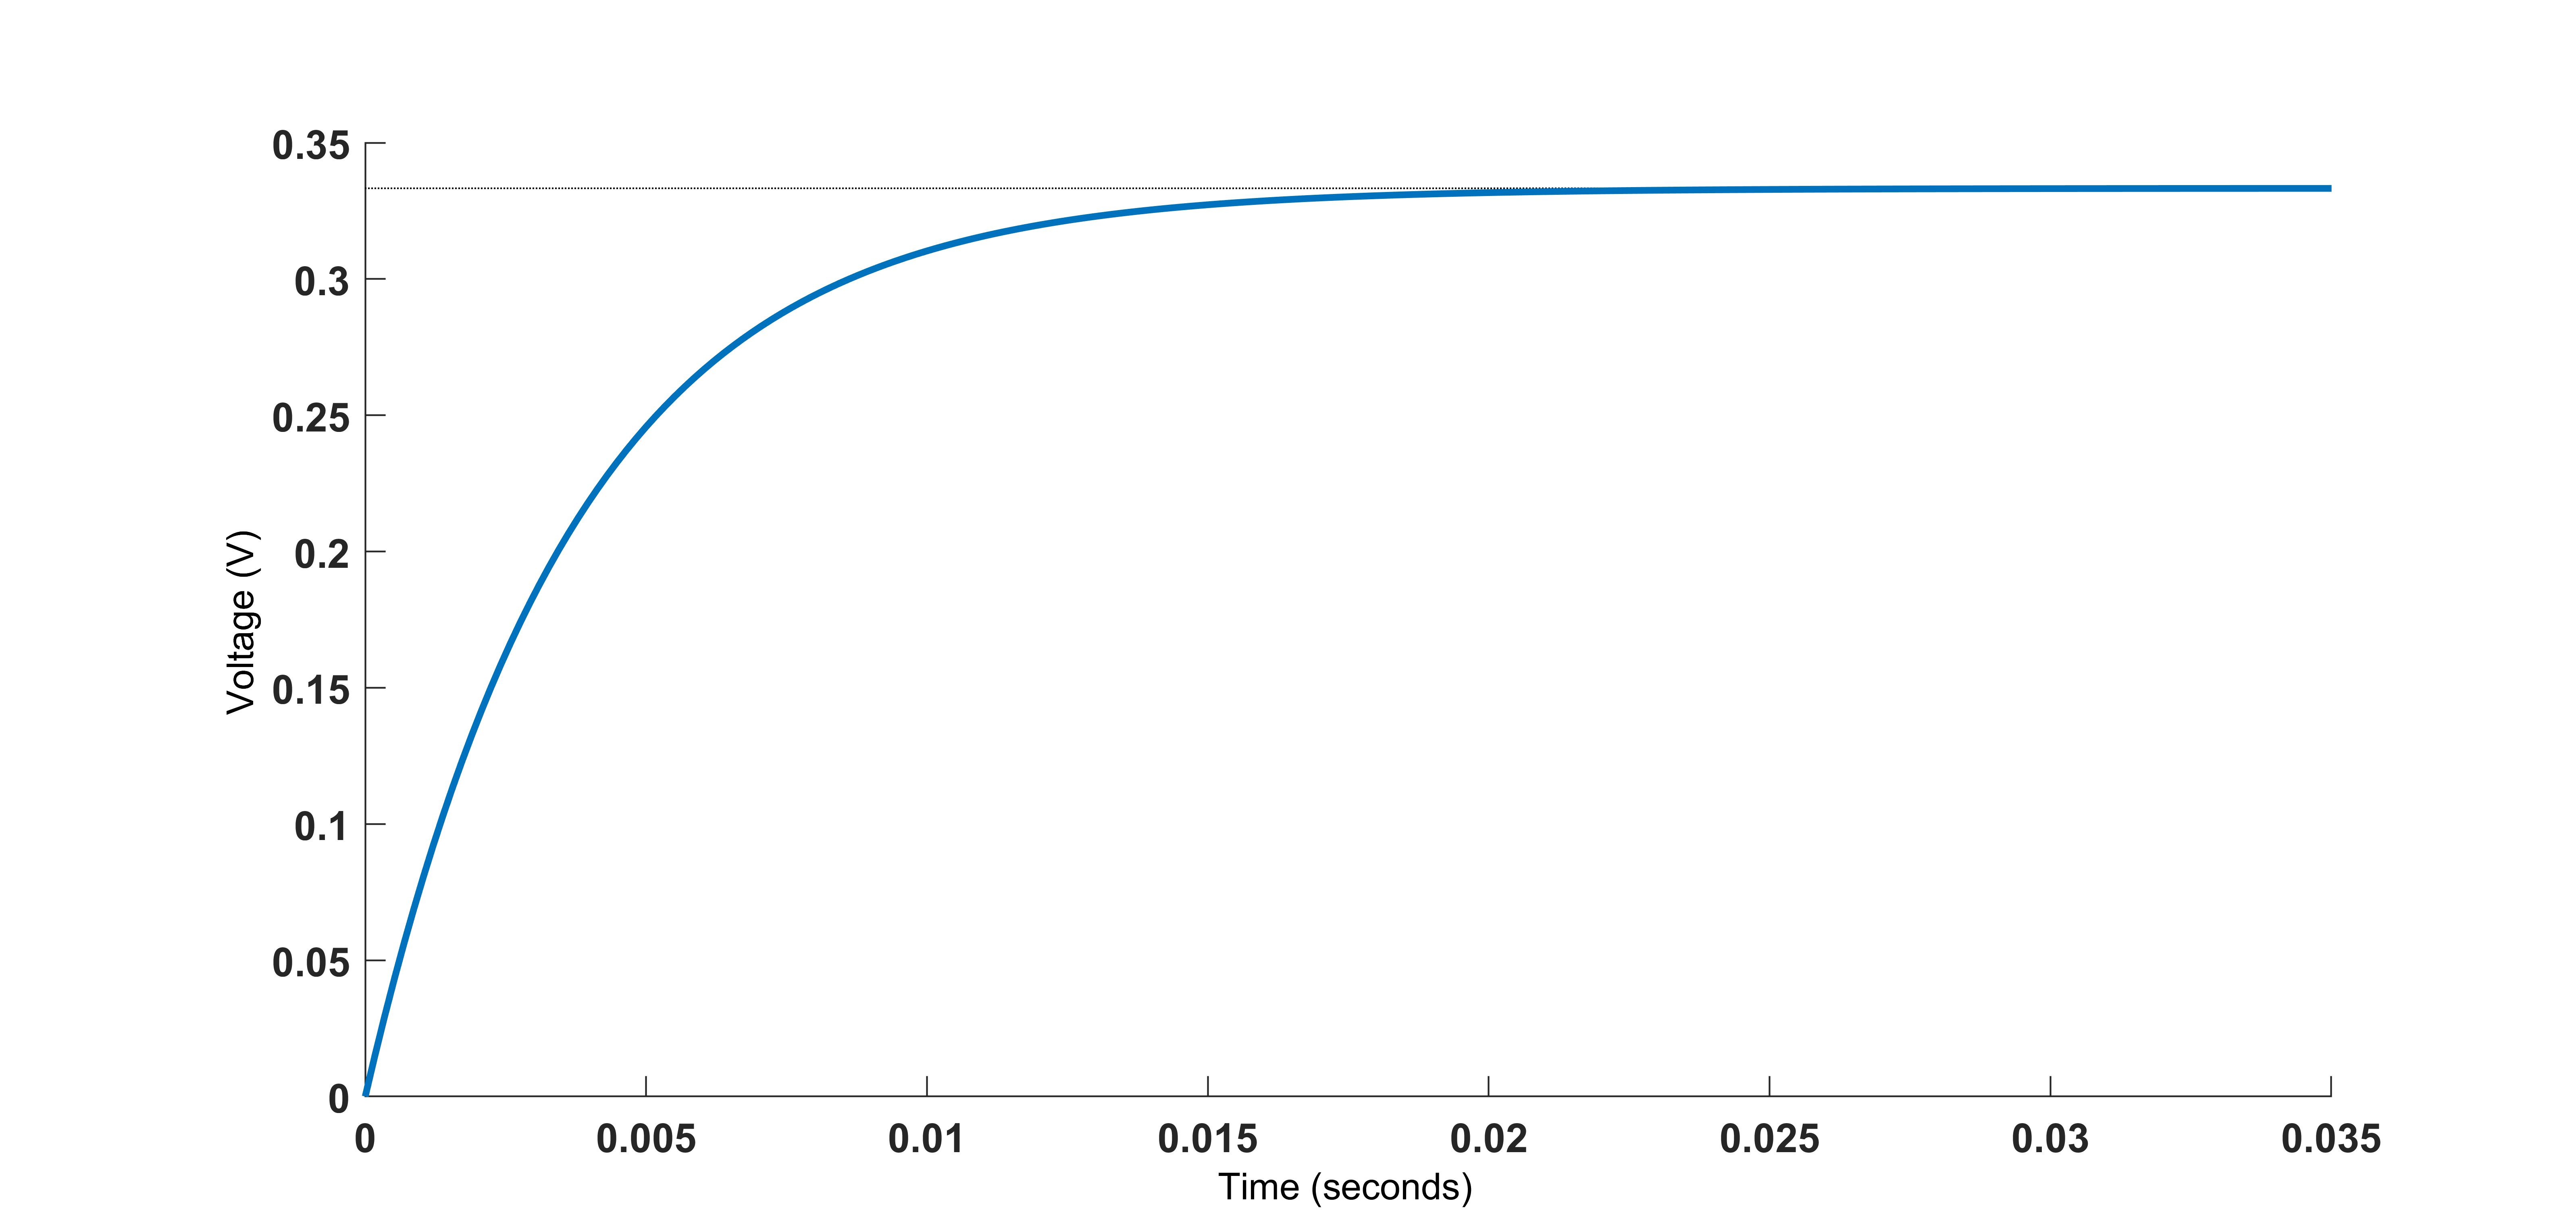
\includegraphics[width=15cm]{step.jpg}
        \caption{Step input plot of the system using Matlab. The gain of the system is 1/3.}
    \end{figure}
    From the plot and Matlab, the gain of the system is 1/3 voltage with a rise time of
    about 0.0082; a pretty fast response time.
    \item Bode plot\\
    The bode plot showed that the system is a low pass filter
    \begin{figure}[h]
        \centering
        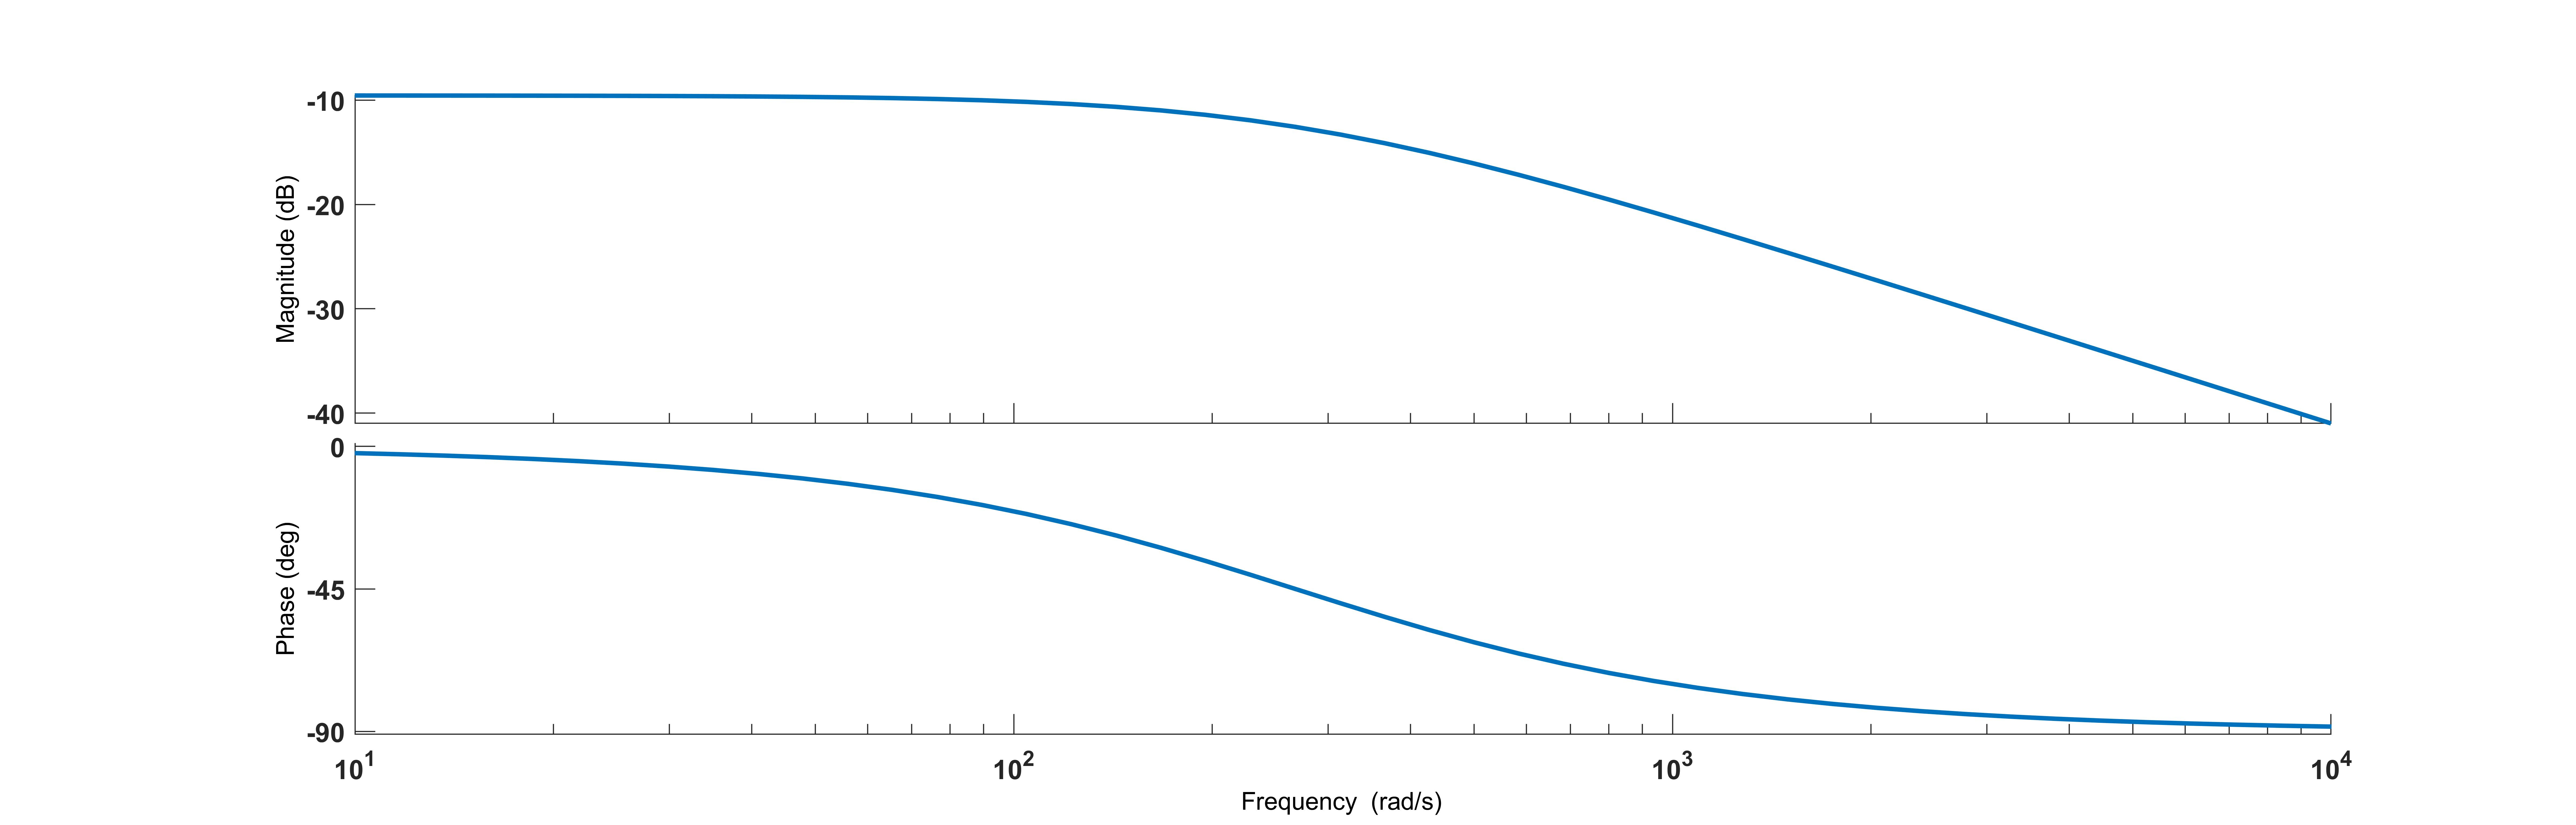
\includegraphics[width=15cm]{bode.jpg}
        \caption{Step input plot of the system using Matlab. The gain of the system is 1/3.}
    \end{figure}
    The cut off frequency of the system is Wn=100 rad/s. The system can 
    perform steadily at frequency bellow the cuf of frequency with a constant phase shift 
    of about 90 degrees. From the open loop analysis  of the system, i was found that the 
    gain margin and the phase margin of the system are infinity respectively.
    \item Nyquest Plot\\
    \begin{figure}[h]
        \centering
        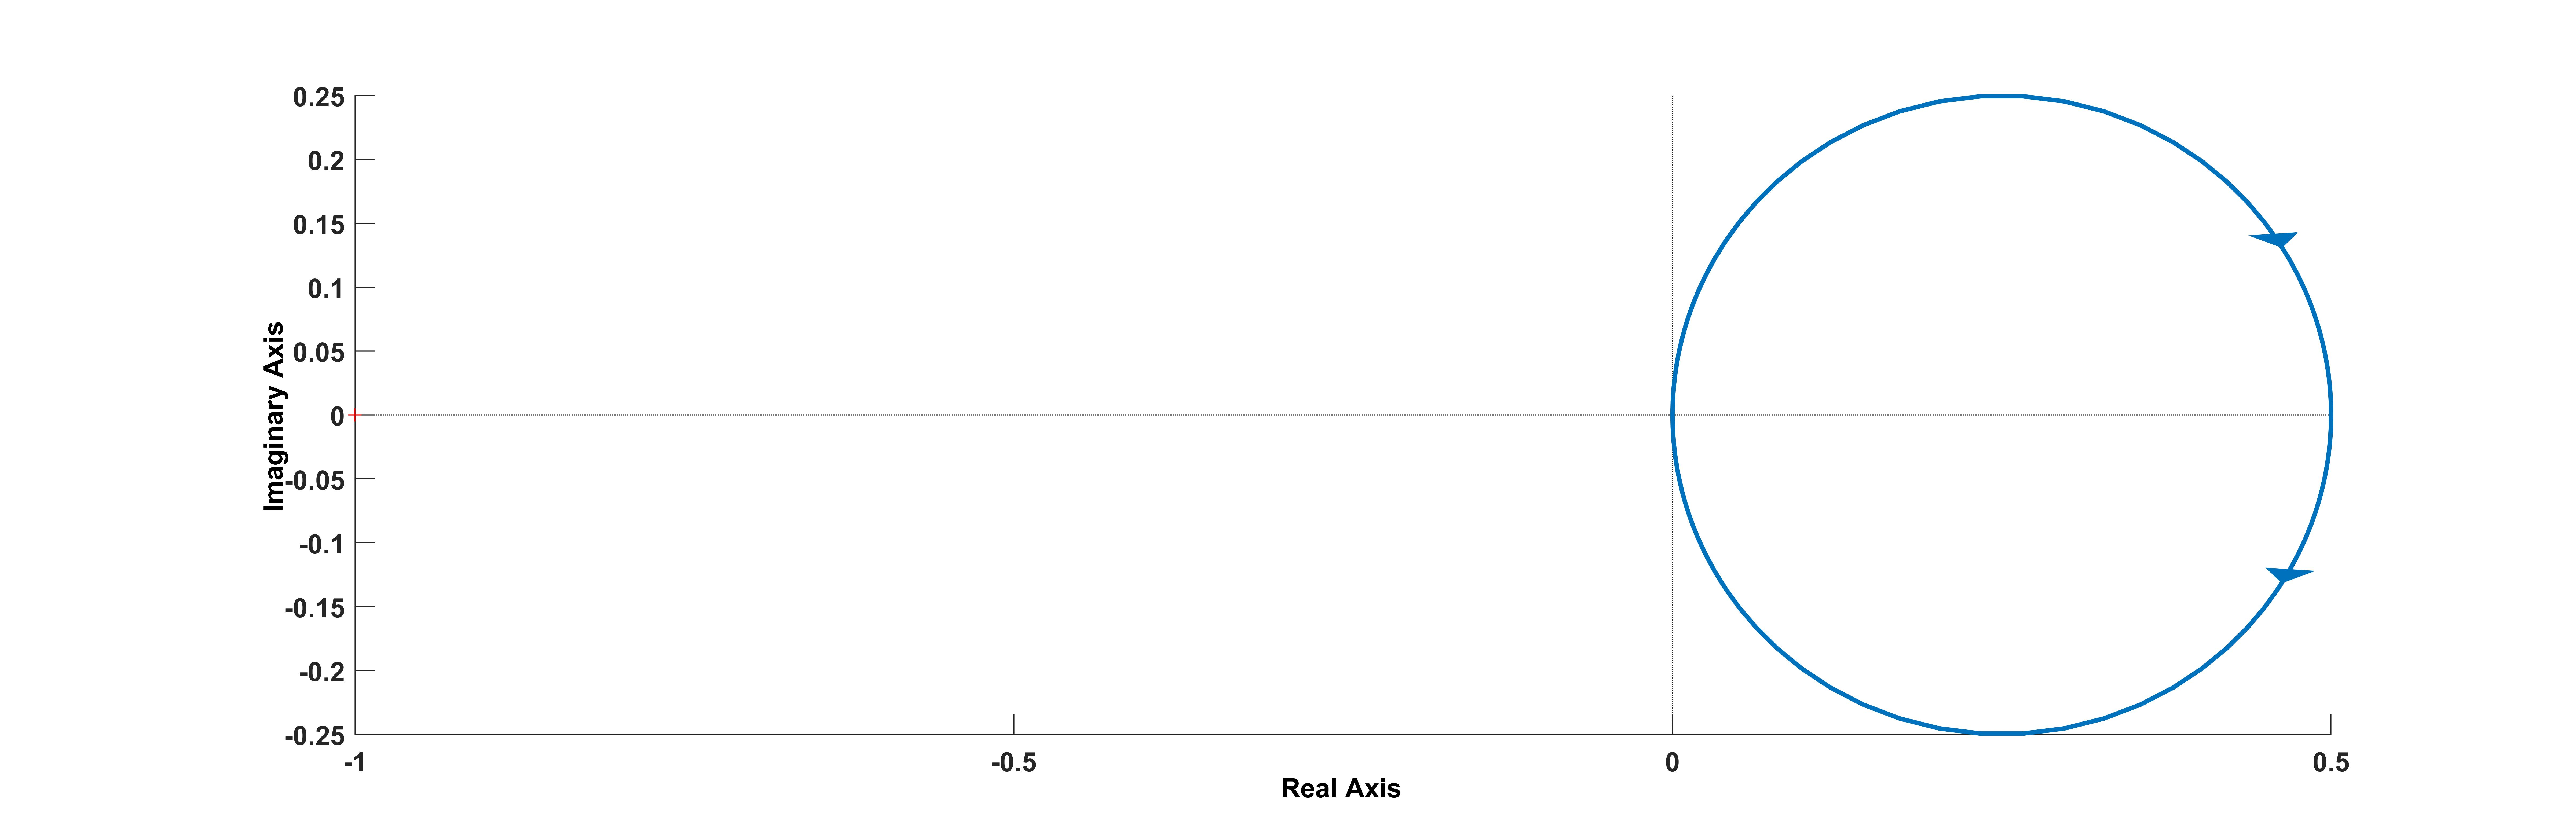
\includegraphics[width=15cm]{nyq.jpg}
        \caption{Nyquest plot of the system using Matlab. The data points are far from the instability point -1 }
    \end{figure}\\
    From the i mage above, our system is stable at pole. The system has not zeros. 
    In addition, the system is also robust as -1 is not encircle and any root on the 
    Nyquest plot is far at safe distance from the -1. 
    \item Root Locus\\
    Below we have the root locus plot of the system
    \begin{figure}[h]
        \centering
        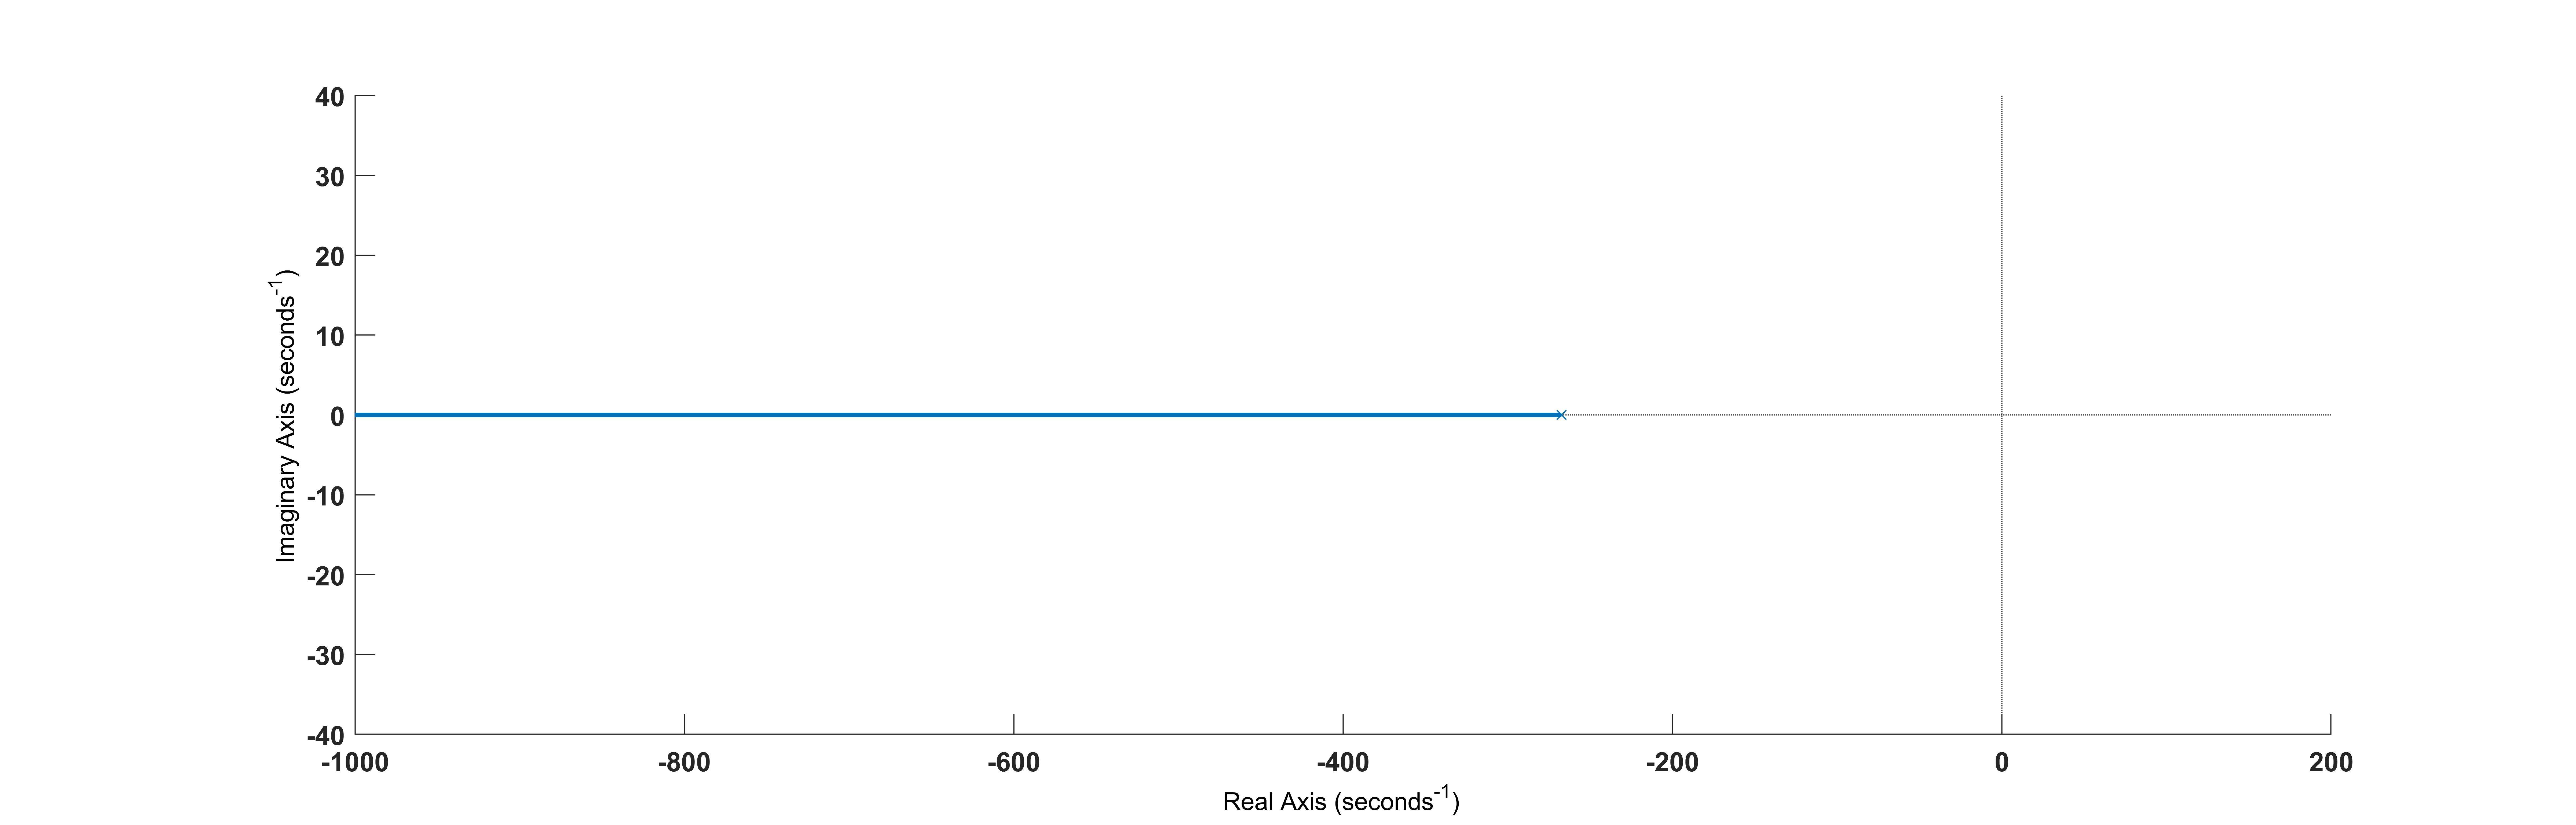
\includegraphics[width=15cm]{rlocus.jpg}
        \caption{Root locus plot using Matlab.}
    \end{figure}\\
    From the plot we can deduct that as the value of k increases, the root of the system 
    goes to negative infinity. This confirm the stability of the system as the root 
    can never get into the right half plan of the plot.
\end{itemize}
\section*{Experimental Results}
Using MyRio, the system was reproduced experimentally using with LabView as showed
in the figure 2. In the diagram, a square wave of the  of 50 percent duty circle.
This wave was input to the circuit through the analog output of the MyRio. The 
voltage across the capacitor in the circuit is input to the device from the analog input
pin. TO complete the feedback loop, the input to the device is subtracted from the 
square wave input signal and feed back to the system. The data collected is plotted ans showed
in the figure below.\\
\begin{figure}[h]
    \centering
    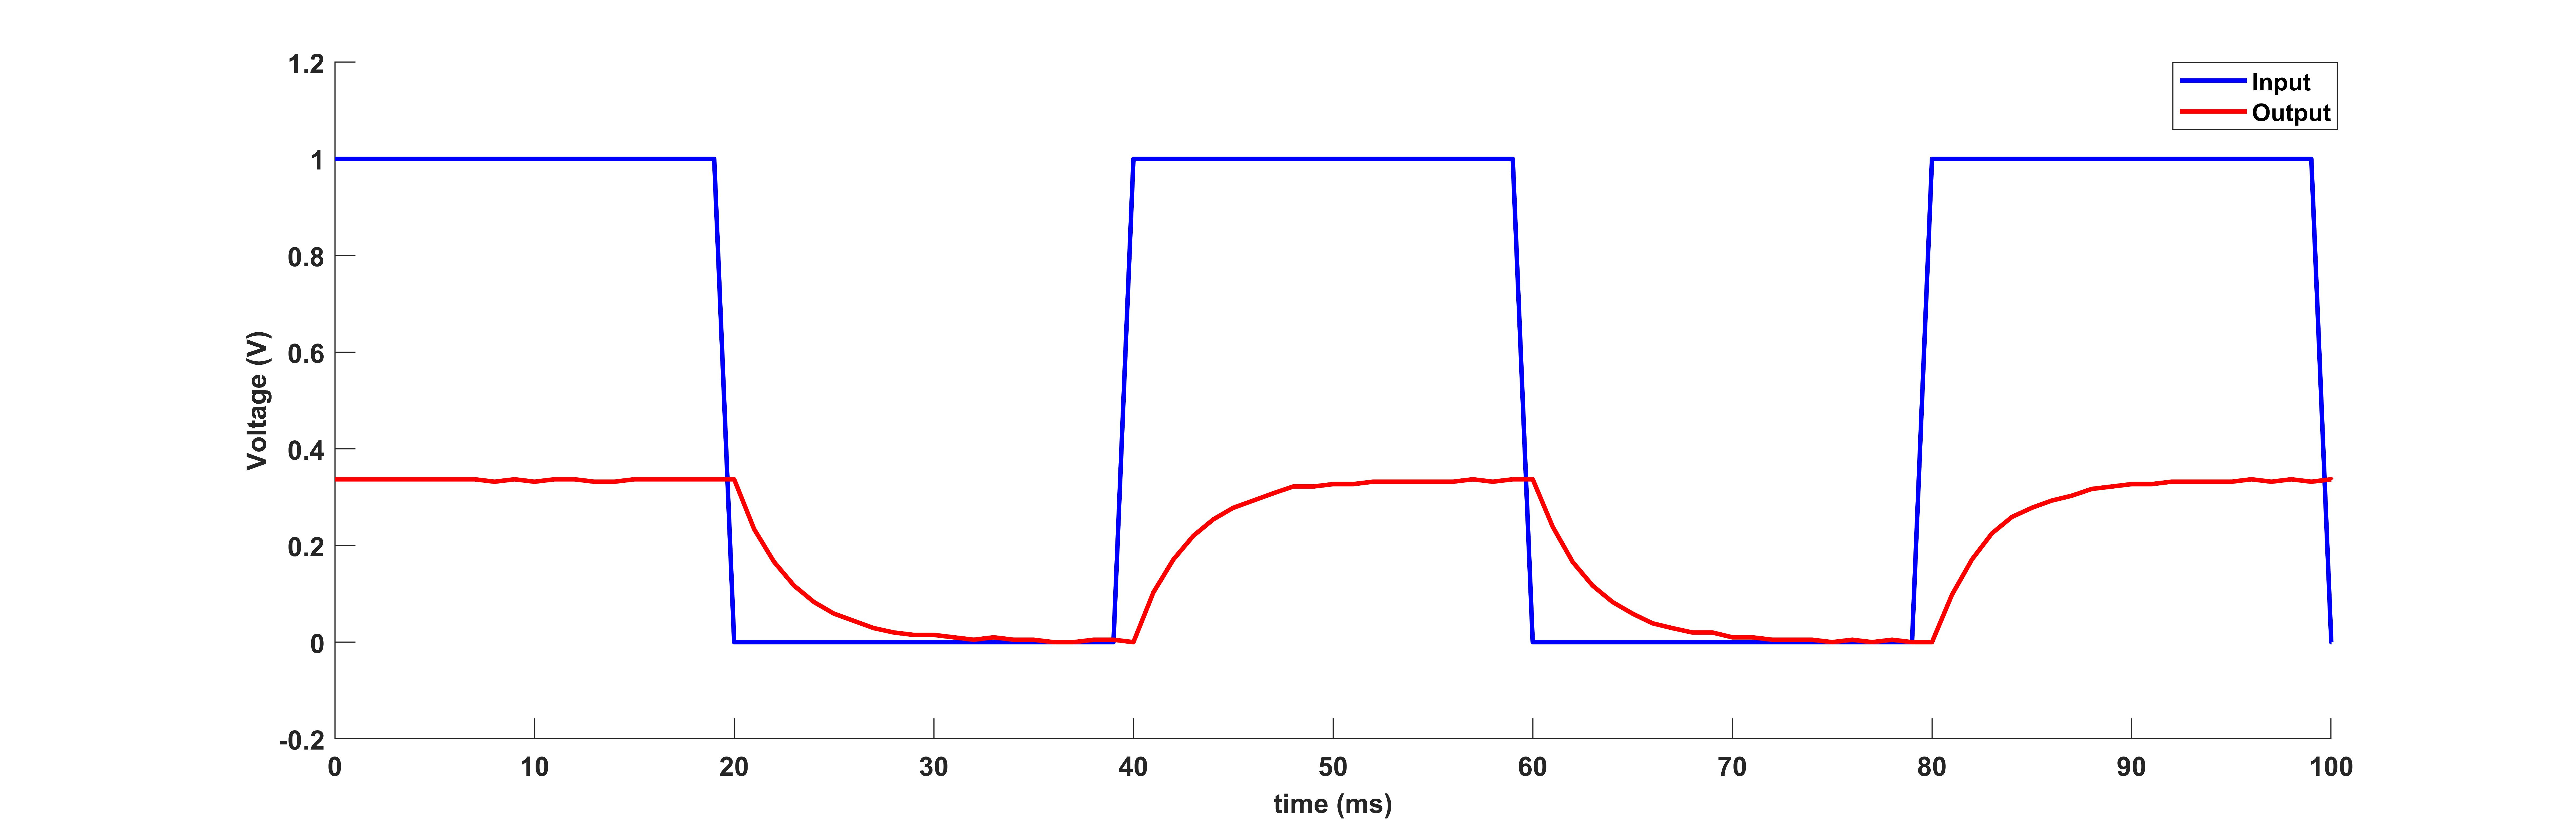
\includegraphics[width=15cm]{expstepin.jpg}
    \caption{Root locus plot using Matlab.}
\end{figure}\\
The gain of the experimental system is .334; a percent of error of
0.3 percent that can be neglected and associated tolerance
in the value of the resistor and capacitor used in the circuit. The 
above plot is generated from a loop that ran for every 1 ms.
To see effected of how wait time of execution of the loop,
Data was recorded at wait time 0f 10 ms and 100 ms. The 10 ms second
wait time plot below shows a difference pattern to the 1 ms plot.\\
\begin{figure}[h]
    \centering
    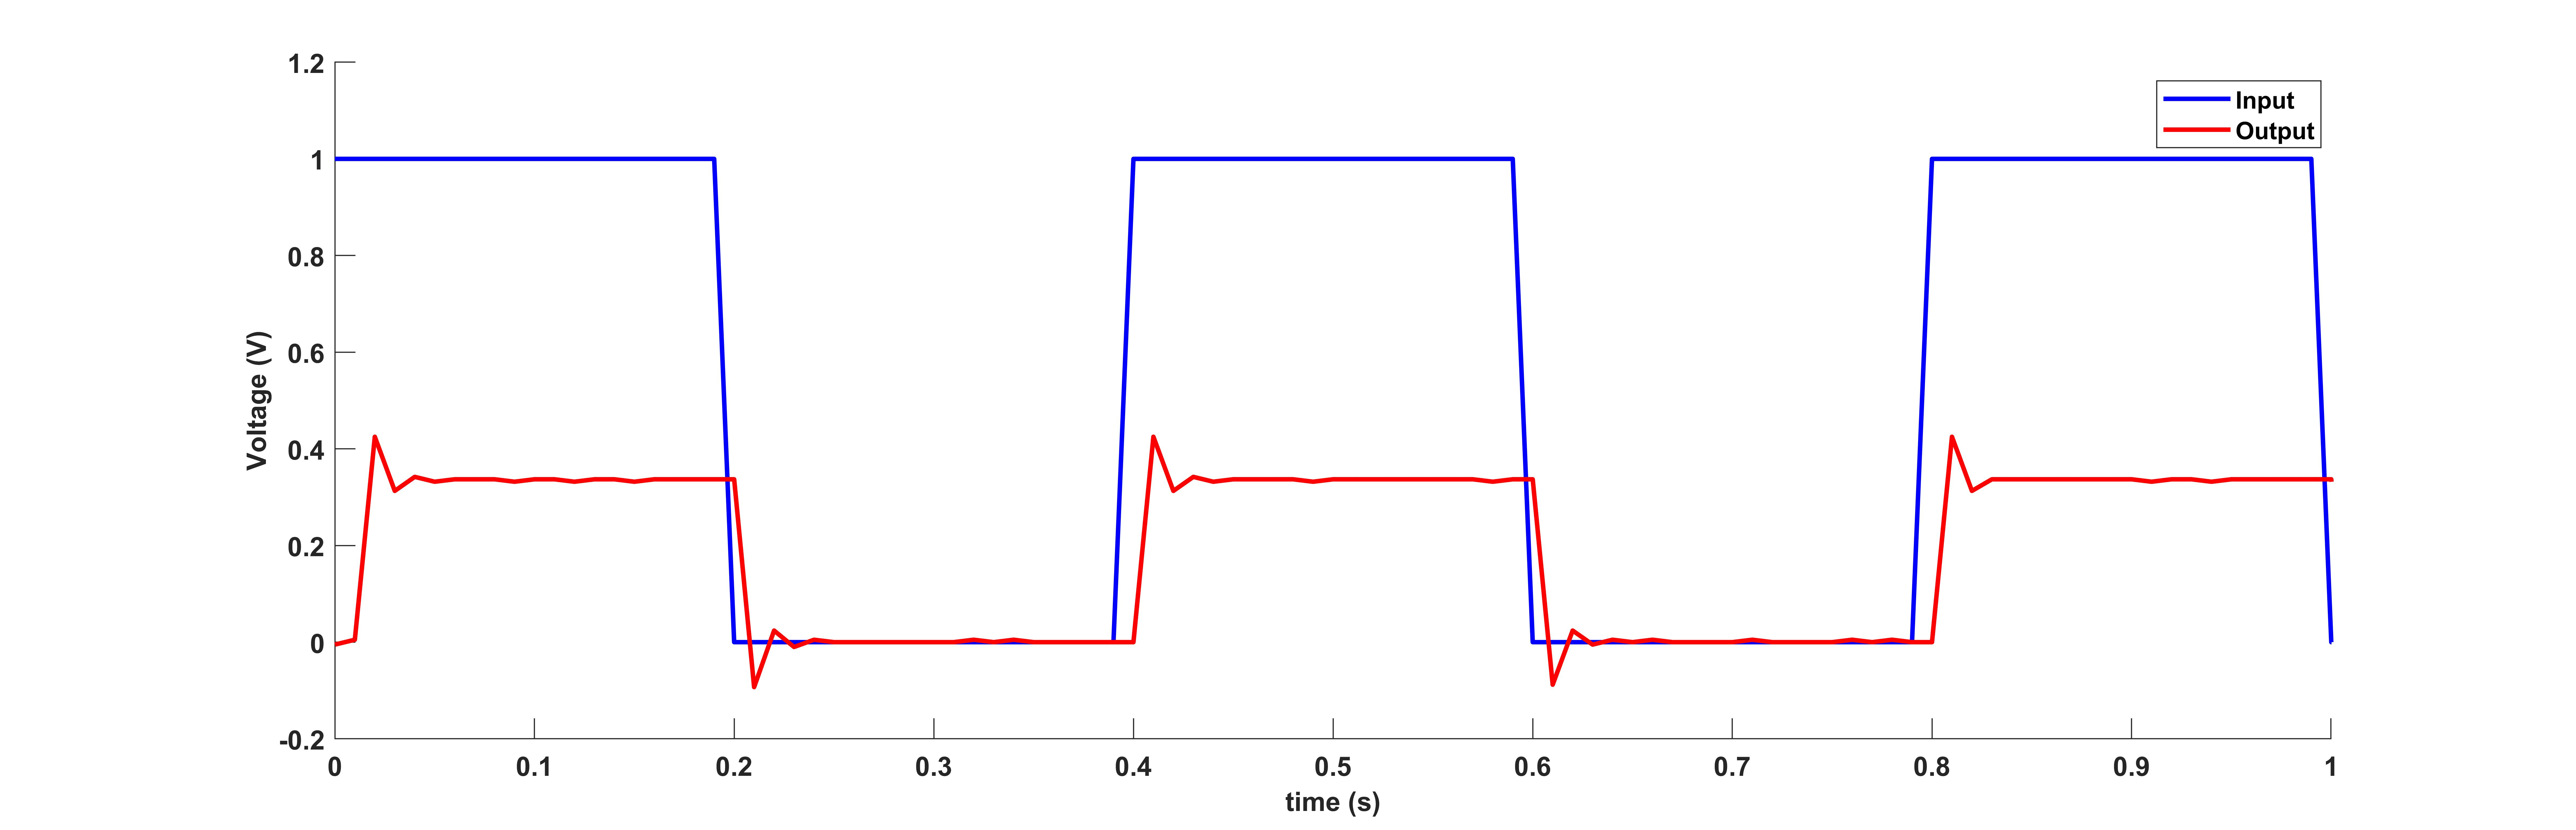
\includegraphics[width=15cm]{expstepin10.jpg}
    \caption{Root locus plot using Matlab.}
\end{figure}\\
In addition, the plot of the 100 ms below is similar to the the 10ms.\\
\begin{figure}[h]
    \centering
    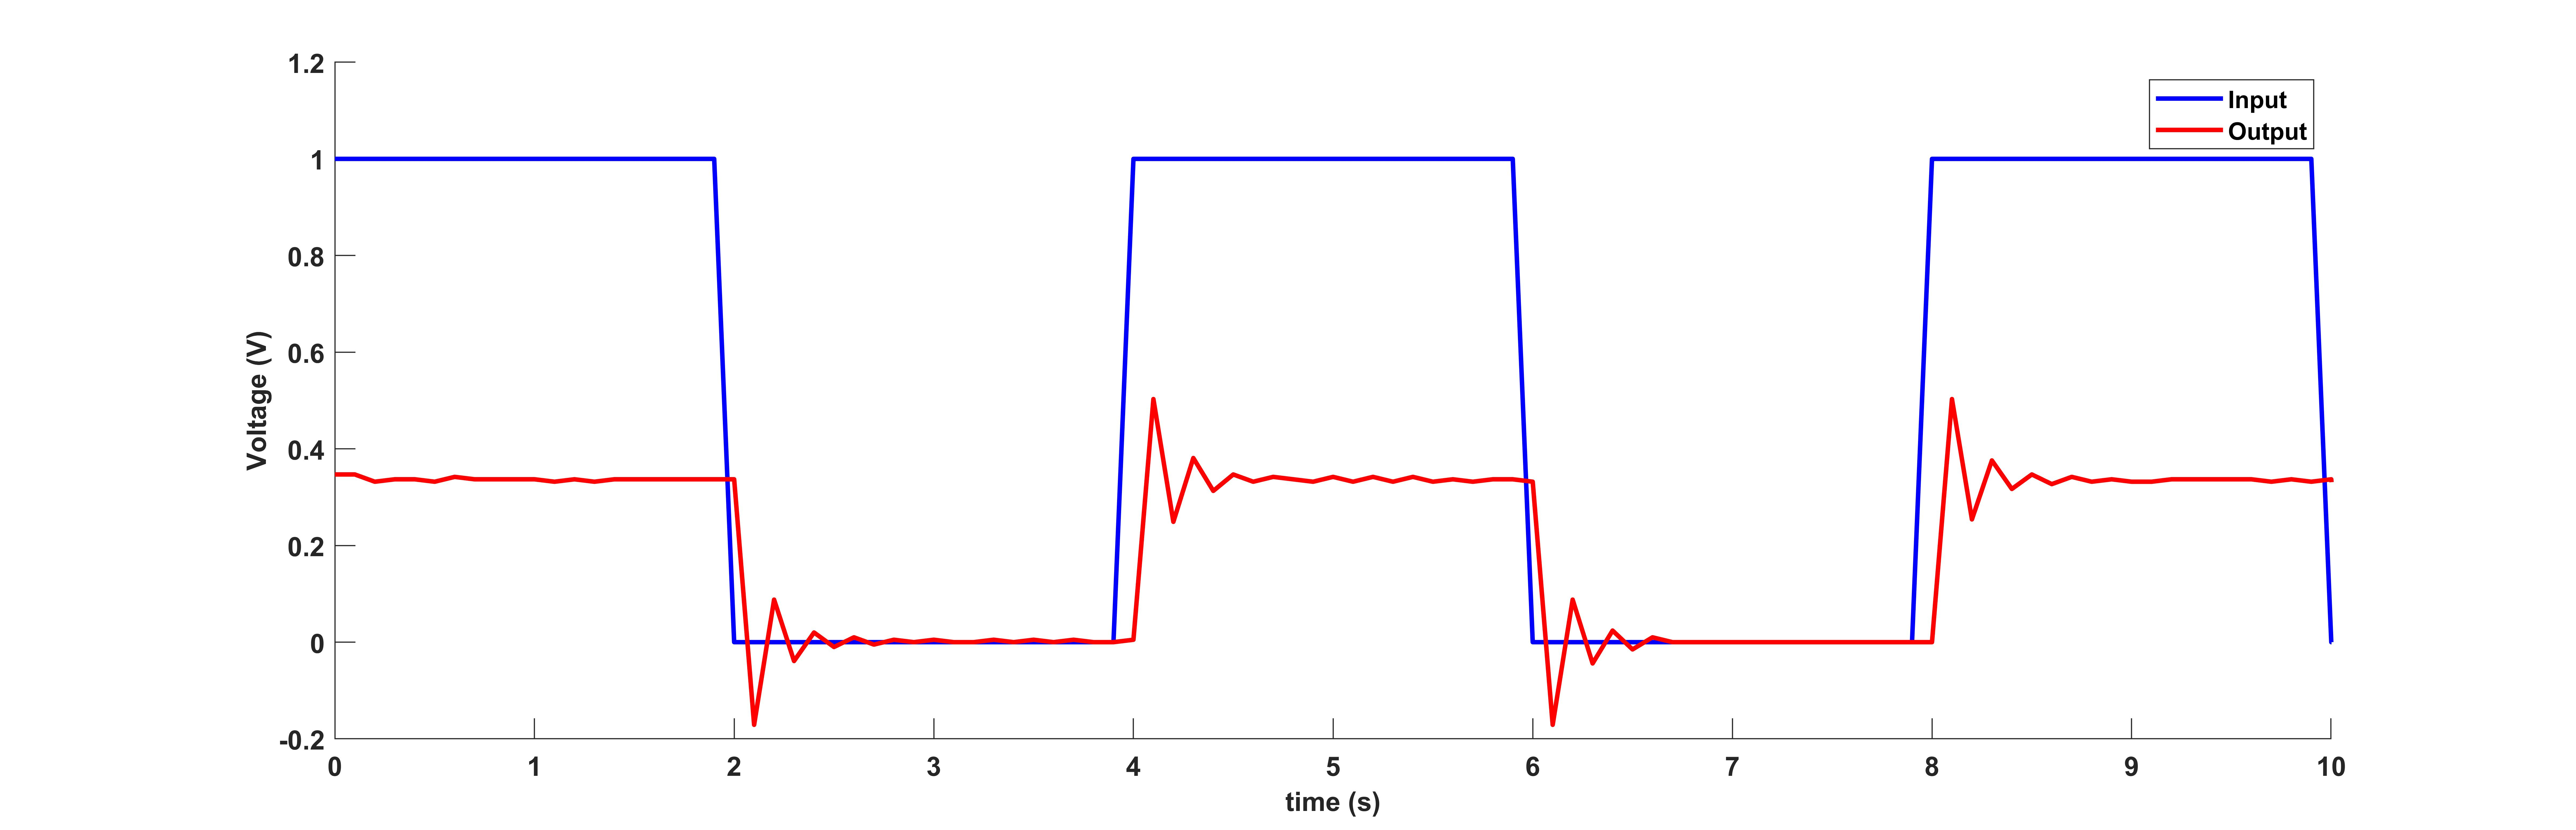
\includegraphics[width=15cm]{expstepin100.jpg}
    \caption{Root locus plot using Matlab.}
\end{figure}\\
The both have an overshot of 0.1. The inconsistency between the 1 ms, 10 ms and 100 ms 
could be due to the resoluton of the data point. As we increase the wait time of the loop,
the recorded data point a less and therefore has lower resolution on plot.
\section*{Conclusion}
The experimental and theoretical results in this lab show similarities. We obtained
the almost the same gain with a error of les than 0.5 percent. The can conclude that 
our circuit is reliable on the standard of matching the theoretical result with a proportional 
controller of k=1 and a sampling period of 1 ms. The difference in the data 
of the 1 ms and the 10, 100 ms are not explicitly known. We believe it could
be due to the change in the sampling frequency with should impact
the MyRIo sampling ability. \\
Our system is robust. The sta of the system can be confirmed from the Nyquest and root locus
plot.  It was found that, for any value of k, the system will always stay 
stable. However, the limitation in hardware that will be used should be taken 
into consideration\\
It is important to note that though we have a feedback back loop, hour system has gain of  1/3
with an input of 1 which is not desirable because of the huge error. It can be concluded that 
a proportional controller is not the best fit for this kind of circuit 
even though a feedback is used when minimizing error is critical.
\end{document}

